% Copyright (C)  2015  Alexander Jankowski, Philipp Hacker.
% Permission is granted to copy, distribute and/or modify this document
% under the terms of the GNU Free Documentation License, Version 1.3
% or any later version published by the Free Software Foundation;
% with no Invariant Sections, no Front-Cover Texts, and no Back-Cover Texts.
% The lincense itself can be found at <https://www.gnu.org/licenses/fdl-1.3>.

\documentclass[numbers=noenddot,a4paper,notitlepage,twoside,BCOR15mm]{article}
%\documentclass[numbers=noenddot,12pt,a4paper]{scrartcl}

\usepackage[english]{babel}
\usepackage[T1]{fontenc}
\usepackage[utf8]{inputenc}

\usepackage[infoshow]{tabularx}
\usepackage[all]{xy}

\usepackage{amsmath}
\usepackage{amssymb}
\usepackage{units}
\usepackage{upgreek}
\usepackage{esint}
\usepackage{graphicx}
\usepackage{ziffer}

\usepackage{float}
\usepackage{lscape}

\usepackage[labelfont=bf]{caption}
\usepackage{wrapfig}
\usepackage{subcaption}

\usepackage[backref=page]{hyperref}

\usepackage{csquotes}
%\usepackage{ifoddpage}
\usepackage[infoshow]{tabularx}
\usepackage{fancyhdr}

\usepackage{sectsty}
\usepackage{times}

\usepackage{lmodern} %TODO Schriftart

\renewcommand{\headrulewidth}{0.1pt}
\renewcommand{\footrulewidth}{0.1pt}
\newcommand{\name}{\text{Philipp Hacker}} %TODO Name des Protokollanten eintragen

\setlength{\parindent}{0pt}

\newcommand{\degree}{^\circ}
\newcommand{\diff}{\textnormal{d}}
\newcommand{\tenpo}[1]{ 10^{#1}}
\newcommand{\greek}[1]{\greektext#1\latintext}
\newcommand{\ix}[1]{_\text{#1}}
\newcommand{\imag}{\mathbf{i}}
\newcommand{\tilt}[1]{\textit{#1}}
\newcommand{\grad}[1]{\textit{grad}\left(#1\right)}
\newcommand{\divergenz}[1]{\textit{div}\left(#1\right)}
\newcommand{\euler}{\mathnormal{e}}
\newcommand{\fett}[1]{\textbf{#1}}

\title{\fett{\underline{Report:}} XPS - surface analysis} %TODO Name des Versuchs eintragen
\author{Alexander Jankowski, Philipp Hacker}
\date{\today}
\pagestyle{fancy}
\fancyhead[C]{\thepage}
\fancyhead[R]{\name}
\fancyfoot[C]{\thepage}
\fancyhead[L]{Section \thesection}

\begin{document}

\renewcommand*{\equationautorefname}{eq.}
\renewcommand*{\figureautorefname}{fig.}
\renewcommand*{\tableautorefname}{tab.}
\renewcommand*{\sectionautorefname}{sec.}
\renewcommand*{\subsectionautorefname}{sec.}
\renewcommand*{\subsubsectionautorefname}{sec.}
\renewcommand*{\figurename}{Fig. }
\renewcommand*{\tablename}{Tab.}

\renewcommand*{\figurename}{Figure }
\renewcommand*{\tablename}{Table}

\maketitle
\begin{center}
Supervisor: Dr. Robin John\\ %TODO Name des Betreuers eintragen
	Date: 07.01.2016 \\ %TODO Datum des Versuchs eintragen
	\begin{table}[h]
		\centering
		Grade: %TODO Gute Note erhalten :)
		\begin{tabularx}{1.5cm}{|X|}
			\hline \\ \\
			\hline
		\end{tabularx}
	\end{table}
\end{center}
\vspace*{\fill}
\tableofcontents
\vfill
\clearpage

	\section{Motivation}

	In the field of surface analysis physics, the method of \tilt{X-ray photoelectron spectroscopy} \fett{XPS}, or also called \tilt{electron spectroscopy for chemical analysis} \fett{ESCA}, is one of the most important techniques to assemble information about the qualitative chemical, physical and quantifiable properties of the surface of a solid state sample. In an ultrahigh vacuum, a sample is radiated with X-ray. In response,  the solid state body emits a flux of electrons, which is then to be resolved in energy and angle.\\


	\clearpage
	\section{Fundamentals}

		The fundamental background to this procedure is the (external) photoelectric effect, which A. Einstein condensed to the rather simple \tilt{photoelectric equation} in \autoref{eq:photo}. An highly energetic photon of the energy $h\nu$ excites an electron in the sample, which is then likely to escape the hull of its binding atom. Therefor, at least the binding energy $E\ix{B}$ of the electron has to be raised by the X-rays. An excited and then released particle can now move, in dependence to its remaining kinetic energy $E\ix{kin}$ and the sample, through the solid state body and eventually reach the surface of it. Through the scattering of the electron with phonons, plasmons and other electrons, as well as the trunks of the sample, its final kinetic energy when detected by an analysor is also reduced by the \tilt{work function} $\Phi$. This magnitude is specific for any angle, surface, sample and location from which the electron is emitted.

			\begin{align}
				E\ix{kin}=h\nu-E\ix{B}-\Phi \label{eq:photo}
			\end{align}

		Obviously, to detect an electron, the energy of the corresponding photon has to be bigger than the binding energy and the work function combined: $E\ix{B}+\Phi<h\nu=E\ix{ph}$. Hence, there is surplus energy for the electron to move with. As there are many different applications for the techniques and results of XPS, there also arises the need for different photon energies. By that, the scanning depth and spectrum of detected electrons is altered, so which results one yields and how they are to be interpreted can easily be varied through a single change of radiation source. For example, the significant \tilt{K}$\alpha$ line of the anode material Mg (which was used in this experiment) is at $h\nu=\unit[1253,6]{eV}$, as which the same property for Al is around $\unit[1486,6]{eV}$. In addition, there is also \tilt{ultraviolet photoelectron spectroscopy} \fett{UPS} for photon energies $\unit[3\dots124]{eV}$.\\
		If one takes a closer look at the process after the electron absorbed a photon, it is seen that there are three stages in the progress of the particle:

			\begin{enumerate}
				\item Excitation/Absorption $\rightarrow$ dependend of the element $X$, photon energy and the initiall level of the electron (cross section of the interaction)
				\item Transportation of the electron to the surface
				\item Exit from the sample and detection.
			\end{enumerate}

		As allready pointed out, the energy spectrum of the particle flux from the sample contains not only of unscattered electrons. Hence, one yields with the intensity information about the lattice of the solid state bodys atoms, phonons and plasmons. In our case, the scattering inside the sample only contributes to the background noise of the spectrum and reveals no information to the experimenter whatsoever.\\
		In addition to that, small energy shifts due to the superposition in eletronic and atomic states cause the alterartion of single peaks in the spectrum. This effect, which is mainly caused by pollution/oxidation of the surface, is called \tilt{chemical shift} and can vary greatly in dimension and manifestation. Most commonly, the chemical shift changes the binding energy $E\ix{B}$, so that the peak of a characteristic transition in the sample is moved in the energy spectrum.\\
		If ones experiments resolution in terms of electron energy is high enough, even further analysis on the chemical and physical features of the solid state body can be made. For example: transitions in $p$-,$d-$ and $f$-orbitals of electrons are resulting in doublets in the electromagnetic spectrum. This can be distinguished in an energy-resolved electron spectrum.\\
		Another characteristic in the spectrum is the discreet decay of a peak. The cause of that is the scattering of electrons at surface plasmons, which only can carry a defined quantum of energy. Thereby the particle lose a certain amount of kinetic momentum each time the excite a plasmon. A peak, to which the initially emitted electron would have contributed, now adds up to the intensity of an slightly lower, less energetic peak in the spectrum.\\
		Finally, secondary electrons must be taken into account, as there are so called \tilt{Auger-electrons}; as shown in \autoref{img:auger}. Electrons from lower energy levels can also be excited by X-ray, as they leave a hole in the hull of the bulk atom. To that, an electron from a higher state can relax and emit a photon on its way "down". This photon can now also excite an electron from the same atom, causing it to contribute to a lower energy in the spectrum, as it has less remaining kinetic energy. Significantly, the mean width of the intensity peaks of such particles is $\sim\unit[1]{eV}$. This corresponds to a the mean lifetime of the electron-hole-pair in the bulk.


			\begin{figure}[h]
				\centering
				\fbox{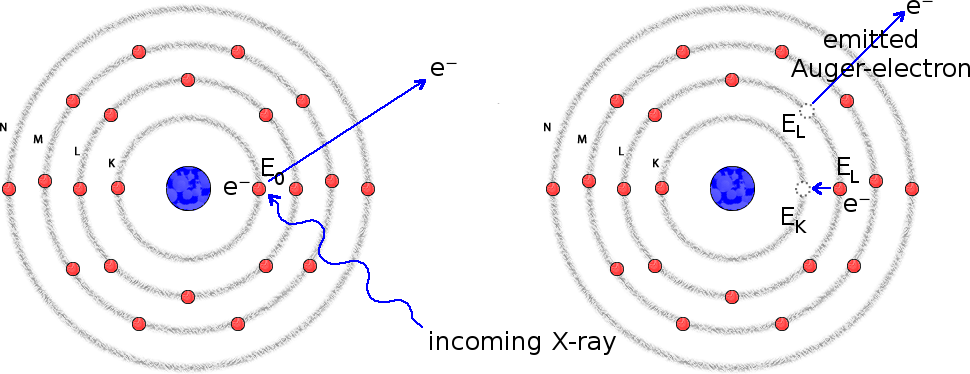
\includegraphics[width=\textwidth]{AES-Combined.png}}
				\caption{AES process. Incoming X-ray excites the atoms and as result emits a photoelectron. Electron in higher energy shell L, moves to shell K. An Auger electron is emitted with a kinetic energy equal to the difference in energy between the transition of shells. \cite{XPSAuger}}\label{img:auger}
			\end{figure}

	\clearpage

		If added up, the electron intensity one yields from the bombardement of a sample with the element $X$ with X-ray $h\nu$ of the intensity $I_{h\nu}$ is equal to \cite{XPSRapha}:

			\begin{align}
				I(E\ix{i},X\ix{i})=&I_{h\nu}T(E\ix{A})A_{\vartheta}\int_{\Omega=0}^{\Omega\ix{0}}\frac{\delta\sigma\ix{X}}{\delta\Omega}\diff \Omega\int_{0}^{d}D\ix{X}(z)\exp\left(-\frac{z}{\lambda\ix{mfp}sin(\vartheta)}\right)\diff z \label{eq:intens} \\
				T(E\ix{A})&: \text{function of transmission of the apparatus} \nonumber\\
				A_{\vartheta}&: \text{adjusted surface of the sample towards the detector, at an solid angle } \Omega\, ,\,\,\vartheta \nonumber\\
				E\ix{i}&: \text{energy level i} \nonumber\\
				D\ix{X}(z)&: \text{density of electrons at the depth of the sample } z \nonumber\\
				\sigma\ix{X}&: \text{cross section of interaction between an electron at} E\ix{i}\, ,\,\, h\nu \nonumber
			\end{align}

		An anticipated spectrum is shown for example in \autoref{img:spektr}.

		\paragraph{Further Properties}

			What one photon, or vice versa an electron, contributes to and what the experimenter detects, varies strongly witht the depth the information is coming from. An X-ray photon penetrates the solid state body by a few $\unit{\mu m}$, while an electron only travels mostly a couple of $\unit{\AA}$ before it gets scattered inside the sample. The Intensity of the unperturbed electron which exit the bulk is best described by a statistical relation such as \tilt{Lamber-Beer} \cite{XPSRa}:

				\begin{align}
					I\ix{e}(\lambda\ix{mfp})\propto\exp\left(-\frac{z}{\lambda\ix{mfp}}\right)\,\, .\label{eq:weg}
				\end{align}

			This concludes to a penetration depth, from which one would still be able to detect an electron from to approximately $d\sim3\lambda\ix{mfp}$. The mean free path of such a particle depends strongly on its energy, the sorroundings and direction it travels. Experimental results for different metals and the excitation depths, as well as corresponding energies is shown in \autoref{img:tiefe}.

				\begin{figure}[h]
					\centering
					\fbox{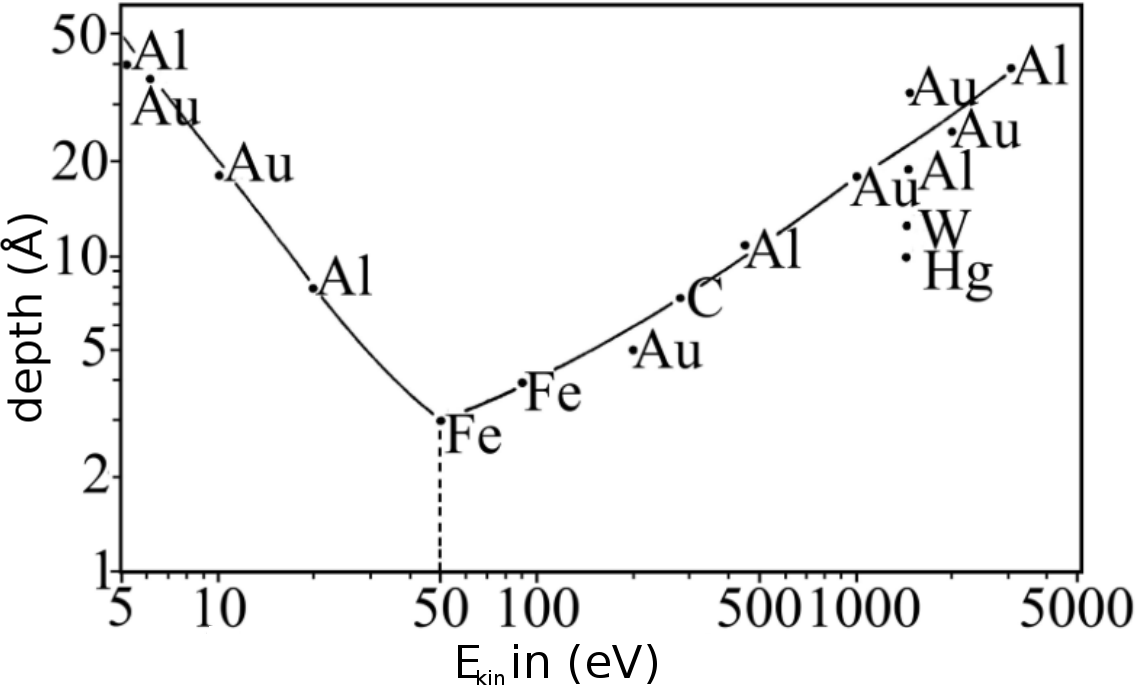
\includegraphics[width=0.75\textwidth]{depth.png}}
					\caption{Exit depths of different metals over kinetic energy.\cite{XPSalt}}\label{img:tiefe}
				\end{figure}

			In such metals with the monolayer thickness $a$ the mean free path of an electron can be described by \cite{XPSRapha}

				\begin{align}
					\lambda\ix{mfp}=\frac{538\cdot a\unit{[nm]}}{(E\ix{kin}\unit{[eV]})^2}+0,41\cdot a^{3/2}\unit{[nm^{3/2}]}\sqrt{E\ix{kin}\unit{[eV]}} \,\,.\label{eq:mfp}
				\end{align}

			A quantitative - say how much of which element is on the sample - analysis can be achieved by a comparison of peak areas $A\ix{i}$ in the spectrum one yields from a full measurement. As there are different probabilities of electron emission for each element $i$, the calculated peak area has to be weighted with the atomic sensitivity facto $ASF\ix{i}$. The concentration of an element on the samples surface is then represented by:

				\begin{align}
					c\ix{i}=\frac{A\ix{i}\cdot ASF\ix{i}^{-1}}{\sum_{j}A\ix{j}\cdot ASF\ix{j}^{-1}} \,\,.
				\end{align}

	\clearpage
	\section{Realisation and Execution}

			\begin{figure}[h]
				\centering
				\fbox{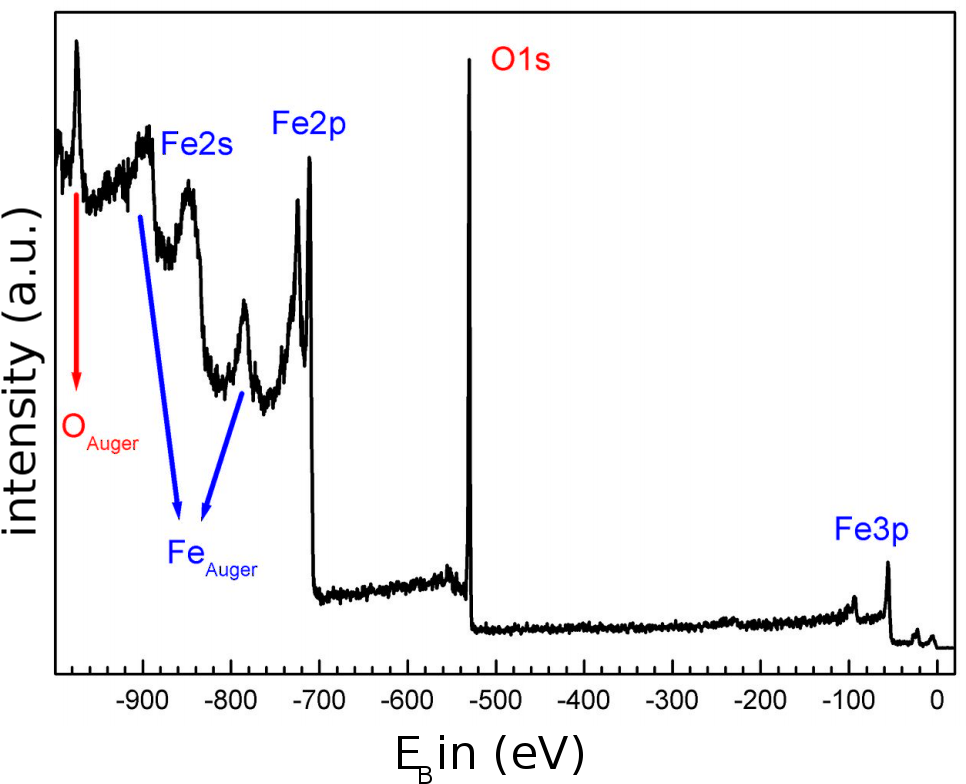
\includegraphics[width=0.6\textwidth]{spectr.png}}
				\caption{Examplary spectrum of magnetite Fe$_3$O$_4$.}
				\label{img:spektr}
			\end{figure}

		The used apparatus consists of a ultrahigh vacuum chamber, in which a pressure of around $\unit[\tenpo{-8}]{mbar}$ is kept, an X-ray canon with the anode material Mg and an detector. The sample, a silicium waver, was allready inserted. Inside the X-ray canon, not-monochromatic radiation is generated by accelerating electrons towards an anode with serverel $\unit{keV}$ of kinetic energy. There they excite another electron, which then exits the bulk and leaves a hole in the shell. This hole is then filled with an electron from a higher position under emission of the characteristic radiation of the bulk material. The spectrum also consists of bremsstrahlung.\\
		By the X-ray excited and emited electrons hit an analysor, after they successfully exited the sample.\\

			\begin{figure}[h]
				\centering
				\fbox{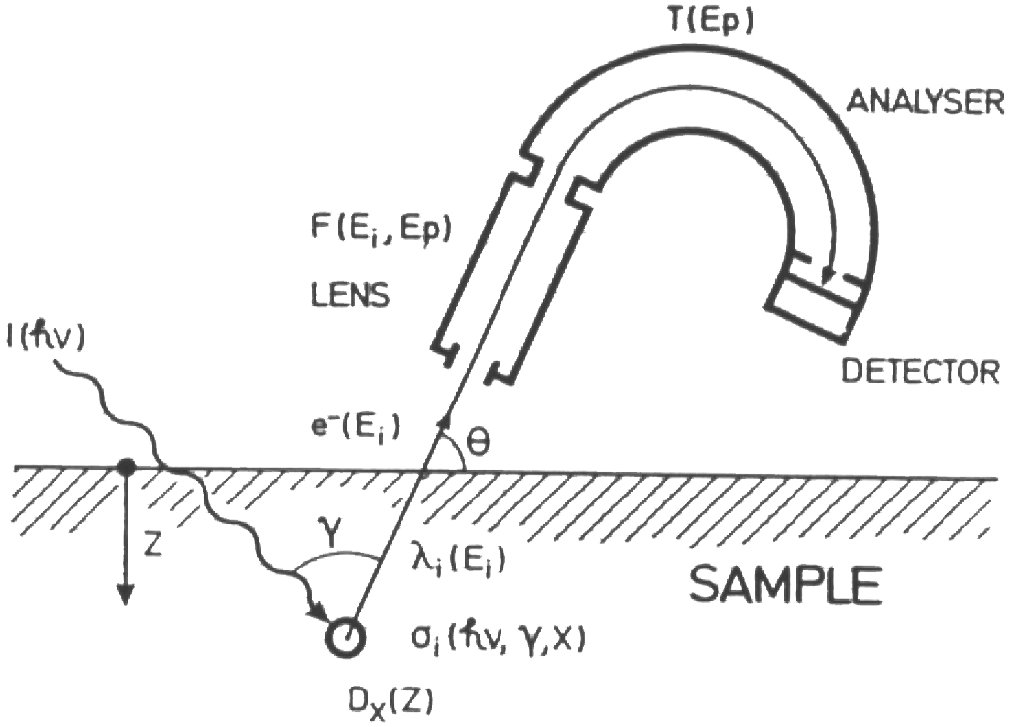
\includegraphics[width=0.6\textwidth]{aufbau.png}}
				\caption{Scheme of the experiments realisation, with the magnitudes from \autoref{eq:intens} included. \cite{XPSRapha}}.
				\label{img:aufbau}
			\end{figure}

		After the experimenter made himself familiar with the apparatus, an overview spectrum was obtained. By that one could easily determine - with the help of certain literature for XPS - the important properties of the sample. In a loop over 30 iterations, the peaks at $\unit[722]{eV}$, $\unit[1158]{eV}$ and $\unit[969]{eV}$ for oxygen, carbon and silicium where measured more accurately.\\
		The pass-energy was set to $\unit[50]{eV}$, the spectrum was $\unit[0\dots1253]{eV}$, the step $\unit[0,05]{eV}$ and the dwell 0,05.

	\clearpage
	\section{Analysis}
	
	\clearpage
	\section{Appendix}

		\bibliography{all.bib}
		\bibliographystyle{unsrt}

\end{document}